Next, we consider the case of a counting Bloom filter. In this setting, an update to add an element increments each of the counters mapped to by the hash functions, with some maximum ceiling $c$ above which the counter cannot increase. A Bloom filter would then just be a counting Bloom filter with a maximum counter value of 1, but we make the additional change that a counting Bloom filter can perform delete operations which work by hashing the element and decrementing the counters at those indices.

Because a counting filter without deletion behaves identically (in terms of responding to queries) to a standard Bloom filter, any attack on a Bloom filter can be trivially converted into an attack against a counting filter simply by performing the exact same operations in the same order. This means that the adversarial advantage against a counting filter, under any of the correctness notions and using any parameters, is bounded below by the advantage against a Bloom filter with the same parameters.

This lower bound is not tight, however, since there are some attacks which exploit the more powerful $\UPO$ oracle provided to the adversary in the case of a counting filter. Consider the public-representation case for an example, where we suppose the structure makes use of a per-representation salt. With a counting filter, the adversary is able to construct representations of arbitrary singleton sets using a single $\REPO$ call and multiple $\UPO$ calls. They begin the game by using $\REPO$ to initialize an empty filter. Then, for some each element $x_1, \ldots, x_{|\col|}$ that the adversary wishes to test, they may first use $\UPO$ to insert the element and then use a second $\UPO$ call to delete the element, returning again to an empty filter. After determining the representation of each singleton subset of $\col$, they can again find $\setT$, $\setR \subseteq \col$ offline computations, where each element of $\setR$ is a false positive for the representation of $\setT$. Since there is only a single representation being manipulated, the salt is in fact constant across the entire experiment. This attack requires a single $\REPO$ call to initialize the filter, $2|\col|$ calls to $\UPO$ to test the elements plus an additional $|\setT|$ calls to $\UPO$ to reinsert the elements found to produce false positives, and $|\setR|$ calls to $\QRYO$ to win the experiment.

In order to achieve good security for a counting filter, it is necessary to use the thresholding assumption that insertions are rejected when the proportion of nonzero counters in the filter reaches some limit $p$. Without this assumption, the adversary can attempt to optimize the number of nonzero counters while keeping the size of the filter (in terms of the number of elements stored in the underlying set) below some constant maximum value. For example, if some $x$ is known to be a false positive for two different sets $\col_1$ and $\col_2$, this increases the probability that elements of $\col_1$ are false positives for the filter representation of $\col_2$ and vice versa. However, using the assumption that there is a limit on the allowed number of nonzero counters, we can derive a false positive bound similar to that of a standard Bloom filter.

\begin{theorem}[Correctness Bound for Counting Filters]\label{thm:count-bf-bound}
Fix integers $k, m, n, \lambda, r\geq 0$, a threshold ratio $p \in [0,1]$, and an error function $d$.
  For every $t, q_R, q_T, q_U, q_H \geq 0$, it holds that
  \begin{eqnarray*}
    \Adv{\erreps}_{\struct_\saltybloom,r}(t,&q_R,& q_T, q_U, q_H) \leq \\ && q_R \cdot \left[\frac{q_H}{2^\lambda} + \binom{q_T}{\mu}\left(p+\frac{k\mu}{m}\right)^{k\mu}\right] \,,
\end{eqnarray*}
where $\mu = \lceil r/\max(k \cdot d(0,1), d(1,0)) \rceil$
\end{theorem}

\begin{figure}
  \boxThmBFSaltCorrect{0.48}
  {
    \underline{$\game_0(\advA)$}\\[2pt]
      $\col \getsr \advA^H$; $\setC \gets \emptyset$; $\setB \gets \col$; $\err \gets 0$\\
      $\pub \getsr \Rep[\HASHO](\col)$\\
      $\bot \getsr \advA^{\HASHO,\QRYO,\UPO,\INTO}$\\
      return $(\err \geq r)$
    \\[6pt]
    \oraclev{$\QRYO(x)$}\\[2pt]
      $\setB \gets \setB \cup x$\\
      if $x \in \mathcal{C}$ then return $\bot$\\
      $\setC \gets \setC \union \{x\}$\\
      $a \gets \Qry[\HASHO](\pub, x)$\\
      if $a \neq [x \in \col]$ then $\err \gets \err + 1$\\
      return~$a$
    \\[6pt]
    \oraclev{$\UPO(x,b)$}\\[2pt]
      $\setB \gets \setB \cup x$\\
      $\setC \gets \emptyset$\\
      $a \gets \Qry[\HASHO](\pub, \qry_x)$\\
      if $x \in \setC$ and $b = a \neq [x \in \col]$ then\\
      \tab $\err \gets \err-1$\\
      if $b = 1$ then\\
      \tab $\col \gets \col + \{x\}$\\
      else\\
      \tab $\col \gets \col - \{x\}$\\
      $\pub \gets \Up[\HASHO](\pub,\up_{x,b})$\\
      return~$\bot$
    \\[6pt]
    \oraclev{$\HASHO(x)$}\\
      $\hh \getsr [m]^2$; $\vv \gets \fff(\hh$)\\
      if $T[x]$ is defined then $\vv \gets T[x]$\\
      $T[x] \gets \vv$;
      return $\vv$
  }
  {
    \underline{$\game_1(\advA)$}\\[2pt]
    \oraclev{$\INTO(x,y)$}\\
      if $x \not\in \col$ or $y \not\in \col$ then\\
      \tab return $\bot$\\
      $i \gets 0$\\
      for $h$ in $\HASHO(x)$ do\\
      \tab if $h$ in $\HASHO(y)$ then $i \gets i+1$\\
      return $i$
    \\[6pt]
    \underline{$\game_2(\advA)$}\\[2pt]
    \oraclev{$\UPO(x)$}\\
      if $\QRYO(x)$ and $x \not\in \col$ then\\
      \tab $\err \gets \err + \max(k \cdot d(0,1), d(1,0))$\\
      $\setB \gets \setB \cup x$\\
      $\setC \gets \emptyset$\\
      $a \gets \Qry[H](\pub, \qry_x)$\\
      if $x \in \setC$ and $a \neq [x \in \col]$ then\\
      \tab $\err \gets \err-1$\\
      $\col \gets \col + \{x\}$\\
      $\pub \gets \Up[H](\pub,\up_{x,b})$\\
      return~$\bot$
  }
  {
  }
  {
  }
  \caption{Games 0--3 for proof of Theorem~\ref{thm:count-bf-bound}.}
  \label{fig:count-bf-bound}
\end{figure}

\begin{proof}
Applying lemma~\ref{lemma:errep} and lemma~\ref{lemma:salttorand}, we reduce the $\erreps$ experiment to the $\erreps1$ experiment with a salted hash function replaced by true random sampling from $[m]$ for each of the $k$ distinct hash values. This is given in $\game_0$. In $\game_1$, we account for the possibility that the adversary can glean information about the overlap between sets by querying each of them separately. In particular, we give the adversary an additional oracle $\INTO$ that returns the number of locations in which two elements overlap. However, we constrain $\INTO$ to only return an answer when the element has previously been sent to some other oracle.

Because new $\QRYO$ and $\UPO$ calls are based on random sampling, this does not provide the adversary with any additional information about how additional elements which might be queried, inserted, or deleted in the future might behave. However, any element which is sent to $\QRYO$ or $\UPO$ which acts as a false positive will be immediately recognized as such. Because of this, our next step will be to move to a game $\game_2$ where any insertion of a false positive immediately gives the adversary credit for the worst possible error that could be caused by either inserting or deleting that element.

Define $\delta = \max(k \cdot d(0,1), d(1,0))$ and $\mu = \lceil r/\delta \rceil$. In $\game_2$, we modify the game so that producing a false positive increments $\err$ by $\delta$, but so that elements cannot be removed from the set. Because false negatives can only be produced by deleting false positives, and the deletion of $n$ false positives can only produce as many as $nk$ false negatives, this means that the adversary has no need to cause false negatives. Doing so can only decrease the chances of producing additional errors by reducing the values of counters in the filter, and so this does not decrease the adversary's ability to produce errors. Furthermore, we increase the allowed number of nonzero counters from $mp$ to $mp + k\lceil r/\delta \rceil$. The only way in which not being able to remove false positives can decrease the adversary's effectiveness is if the maximum capacity of the filter is reached. Since each false positive removed causes $k$ nonzero counters to be returned to zero, and the adversary stops after accumulating $r$ errors, an allowance of an extra $k\lceil r/\delta \rceil$ nonzero counters is enough to make up for this.

Since each new element queried from outside $\col$ has its corresponding indices determined by a true random function, the adversary can do no better than maximizing the number of nonzero counters in its attempt to produce false positives. Assuming the adversary is able to achieve a maximum-capacity number of nonzero counters, the probability of any particular counter being nonzero is $(mp + k\lceil r/\delta \rceil)/m = p + \frac{k}{m}\lceil\frac{r}{\delta}\rceil$. Over $k$ total hashes, the probability of a false positive is $\left((mp + k\lceil r/\delta \rceil)/m = p + \frac{k}{m}\lceil\frac{r}{\delta}\rceil\right)^k$. Since the adversary needs to accumulate $\lceil\frac{r}{\delta}\rceil$ errors over the course of $q_T$ queries, the probability of the adversary succeeding in this game is

$$\Prob{\game_2(\advA) = 1} = \binom{q_U + q_T}{\mu}\left(p+\frac{k\mu}{m}\right)^{k\mu}$$

Therefore the advantage of the adversary in the original game is

$$\Adv{\erreps}_{\struct_s,r}(\advA) \le q_R \cdot \left(\frac{q_H}{2^\lambda} + \binom{q_T}{\mu}\left(p+\frac{k\mu}{m}\right)^{k\mu}\right).$$\missingqed

\end{proof}

For concrete error bounds, we assume that $d(0,1) = d(1,0) = 1$, so that $\mu = \lceil r/k \rceil$. The default parameters are the same as in the case of an ordinary Bloom filter.

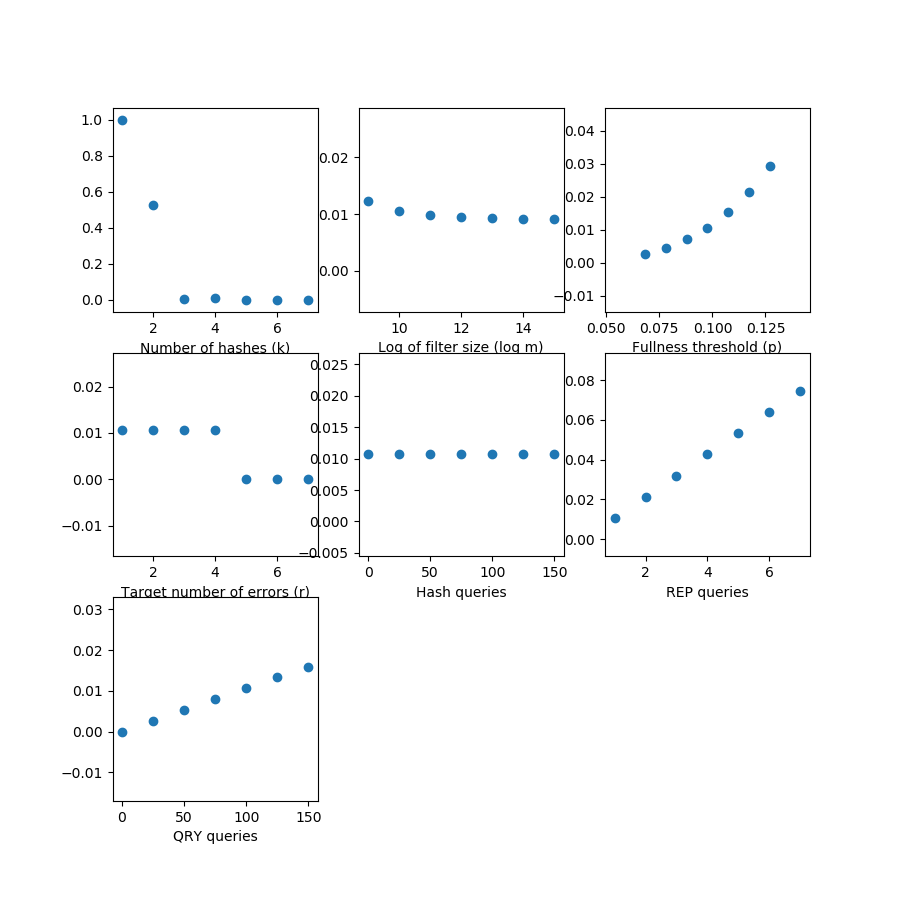
\includegraphics[scale=0.75]{CBF_Fig}

%\subsection{Attack on Counting Filters}

%First, $\advA$ chooses an arbitrary set $\col$ of size $n$ and calls $\REPO$ to get a representation of $\col$. The adversary then chooses $q_U$ distinct elements not in $\col$ and makes a series of $\UPO$ calls to remove each of these from the set. Finally, the adversary chooses up to $q_T$ elements from $\col$ and makes a series of $\QRYO$ calls to test for membership of these elements in the set.

%\begin{tabular}{|l|} 
% \hline
% \underline{adversary $\advA$:}\\
% $\col \gets [n]$\\
% $\REPO(\col)$\\
% for $i \in [q_U]$ do\\
% \tab $\UPO(0,\up_{i+n}')$\\
% for $j \in [q_T]$ do\\
% \tab $\QRYO(0,\qry_{j})$\\
% return 0\\
% \hline
%\end{tabular}